\subsection{Texture Mapping}

Texture Mapping bezeichnet ein Verfahren, welches zweidimensionale Texturen auf ein dreidimensionales Objekt
abbildet. Um die flachen Texturen auf die Oberfläche des Meshs abbilden zu können, muss das Objekt 'UV-unwrapped' werden.
Durch diesen Vorgang wird jedem Punkt auf der Oberfläche des Meshs ein Punkt auf der Textur zugewiesen \parencite{Catmull1974} \parencite{Blinn1976}.
Ein sehr einfaches Beispiel zur Veranschaulichung ist dabei das Würfelnetz.
\textcolor{red}{>>GRAFIK VON WÜRFELNETZ/UV-UNWRAPPING<<}

Texture Mapping sorgt dafür die Objekte 'anzumalen'.
Reale Objekte haben oft sehr detaillierte Oberflächeneigenschaften und sind eigentlich niemals wirklich glatt.
Geometrische Unebenheiten und Feinheiten, wie Kratzer, Rillen und Schmutz lassen sich zwar mithilfe von
Texturen andeuten, jedoch bleibt die Oberfläche komplett glatt. Diese rauhen Oberflächen zu modellieren resultiert
aber in einer deutlich höheren Polygon-Anzahl, was die Performance in großen Szenen schnell negativ beeinflussen kann.
Daher wurden Mapping-Verfahren als Ergänzung entwickelt um die virtuelle Auflösung
solch komplexer Oberflächen kostengünstig zu erhöhen, ohne dabei die Komplexität der Geometrie zu verändern.
Dabei gibt es verschiedenste Shader, welche mithilfe weiterer, spezieller Texturen eine deutlich detailliertere
Oberfläche simulieren können.


% \subsubsection{Normal Mapping}
\subsubsection{Bump Mapping}

Eine Möglichkeit, mit der sich die Oberflächen mit mehr Details rendern lassen, ist das Rendering
mithilfe von sogenannten Bump Maps.
Hierbei werden mithilfe von Texturen, welche zusätzliche Informationen zu den Oberflächen enthalten,
Details generiert, welche den Eindruck einer realistischen Struktur der Oberfläche erzeugen.
Dabei ist es nicht notwendig, dass die Geometrie an sich Informationen dazu beinhaltet \parencite{Blinn1978}.

Bump Maps sind Texturen, basierend auf Graustufen, bei denen die Helligkeit eines Pixels
einen Höhenwert repräsentiert. Schwarz steht mit dem Wert 0 für den tiefsten Punkt und weiß mit dem Wert 1 für den höchsten Punkt.
Eine verbesserte Variante der Bump Maps sind die Normal Maps.
Hier werden die Richtungen der Normalen in jedem Pixel durch einen Vektor repräsentiert,
welcher sich aus den RGB-Werten eines jeden Pixels ergibt. Daraus lassen sich Schattierungen simulieren,
welche kleine Unebenheiten (mit geringer Tiefe) wie Beulen oder Kratzer realistischer aussehen lassen.
Dieser wird aus Lichtquellen, deren Einfallsrichtung und den Normalen aus der Textur berechnet.
Somit wird auch bei geringer Polygonanzahl eine deutlich realistischer aussehende Oberfläche gerendert.
\parencite{Cohen1998}.

Diese Texturen bieten einen sehr kostengünstigen
Ansatz um Tiefe zu simulieren, Shader basierend auf diesen Methoden sind dabei aber stark
blickwinkelabhängig und sehen schnell unnatürlich verzerrt aus.
Von vorne betrachtet funktioniert die Illusion, je spitzer jedoch der Winkel zwischen Betrachter und
Oberfläche wird, desto auffälliger wird die Tatsache, dass die Silhouette des Objekts immer
noch flach ist, da die Geometrie hierbei nicht verändert wird.
Zusätzlich wird die Effektivität von reinem Normal Mapping in VR-Umgebungen aufgrund der Unabhängigkeit vom Betrachtungswinkel
geschwächt. 

\begin{figure}[h!t]
	\centering
	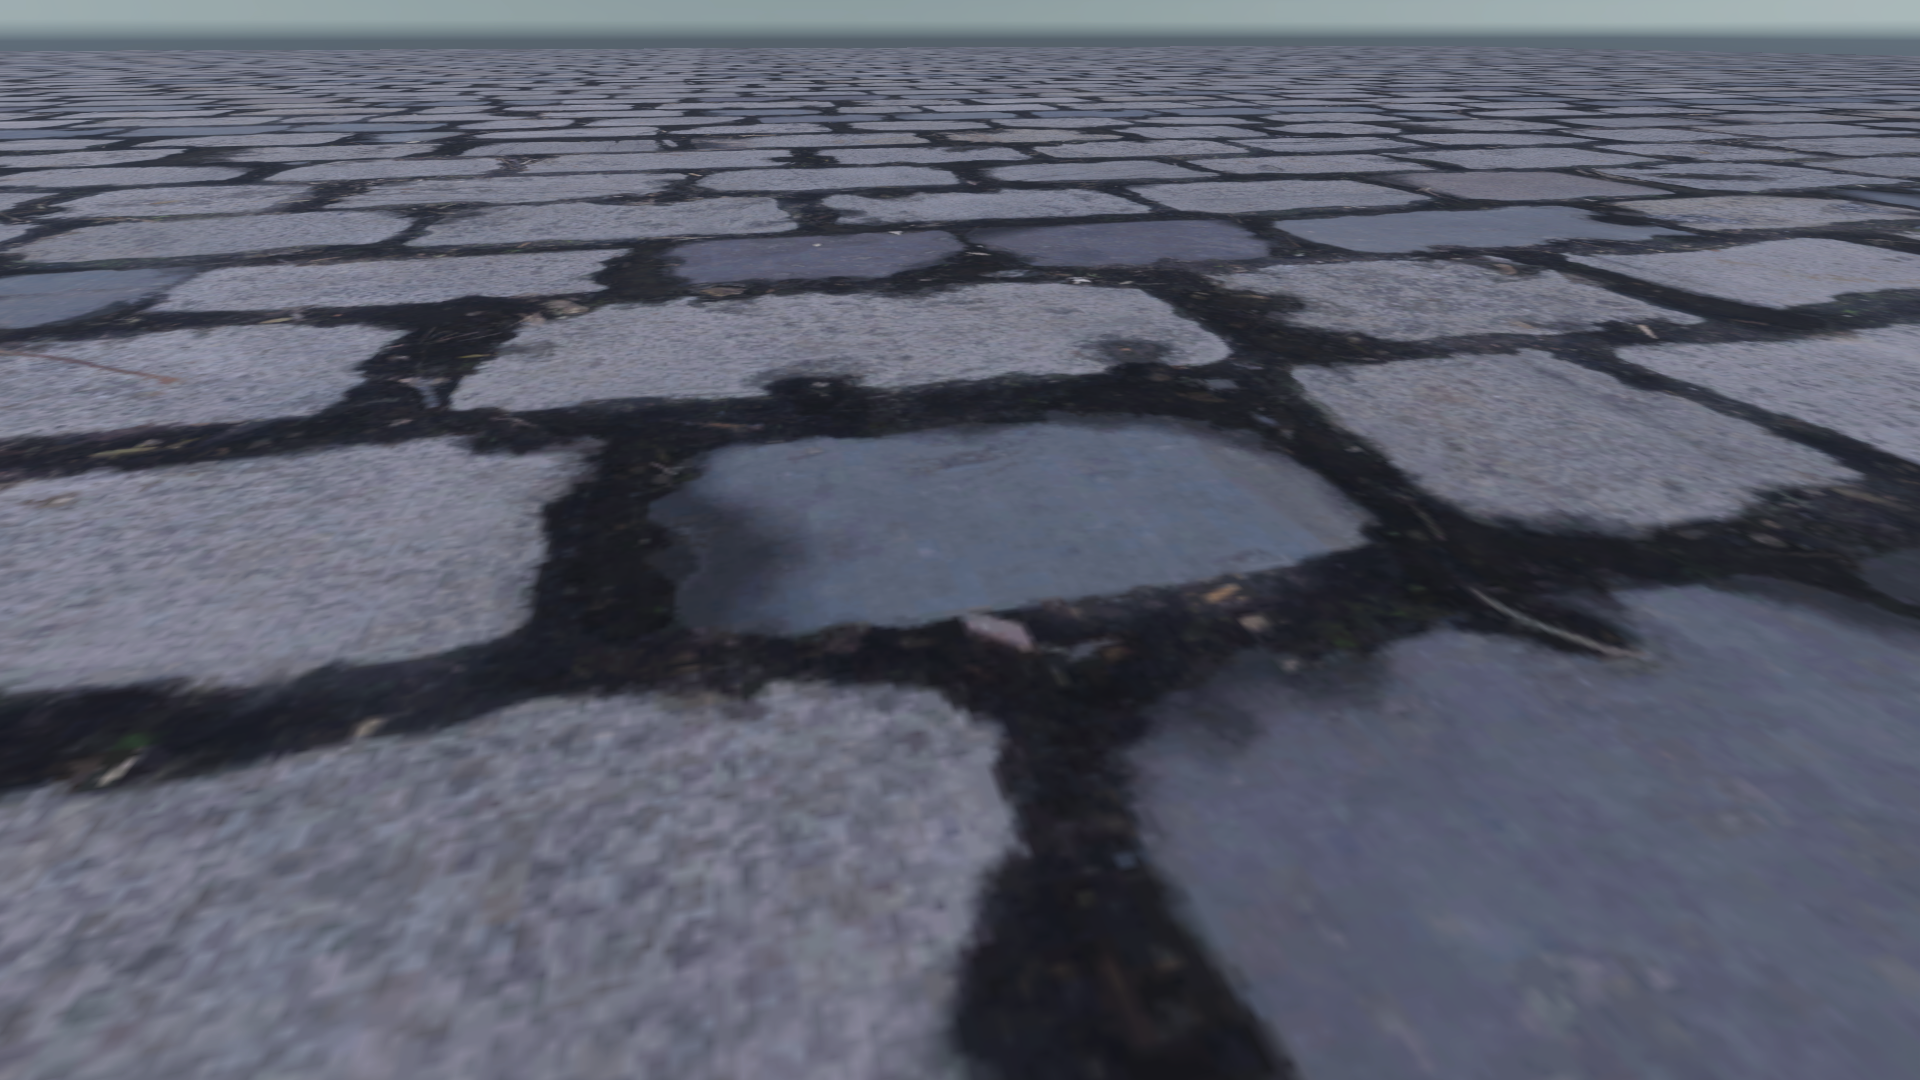
\includegraphics[width=0.49\textwidth]{Grafiken/Basics/Mapping/Vergleich_Diffuse.png}
	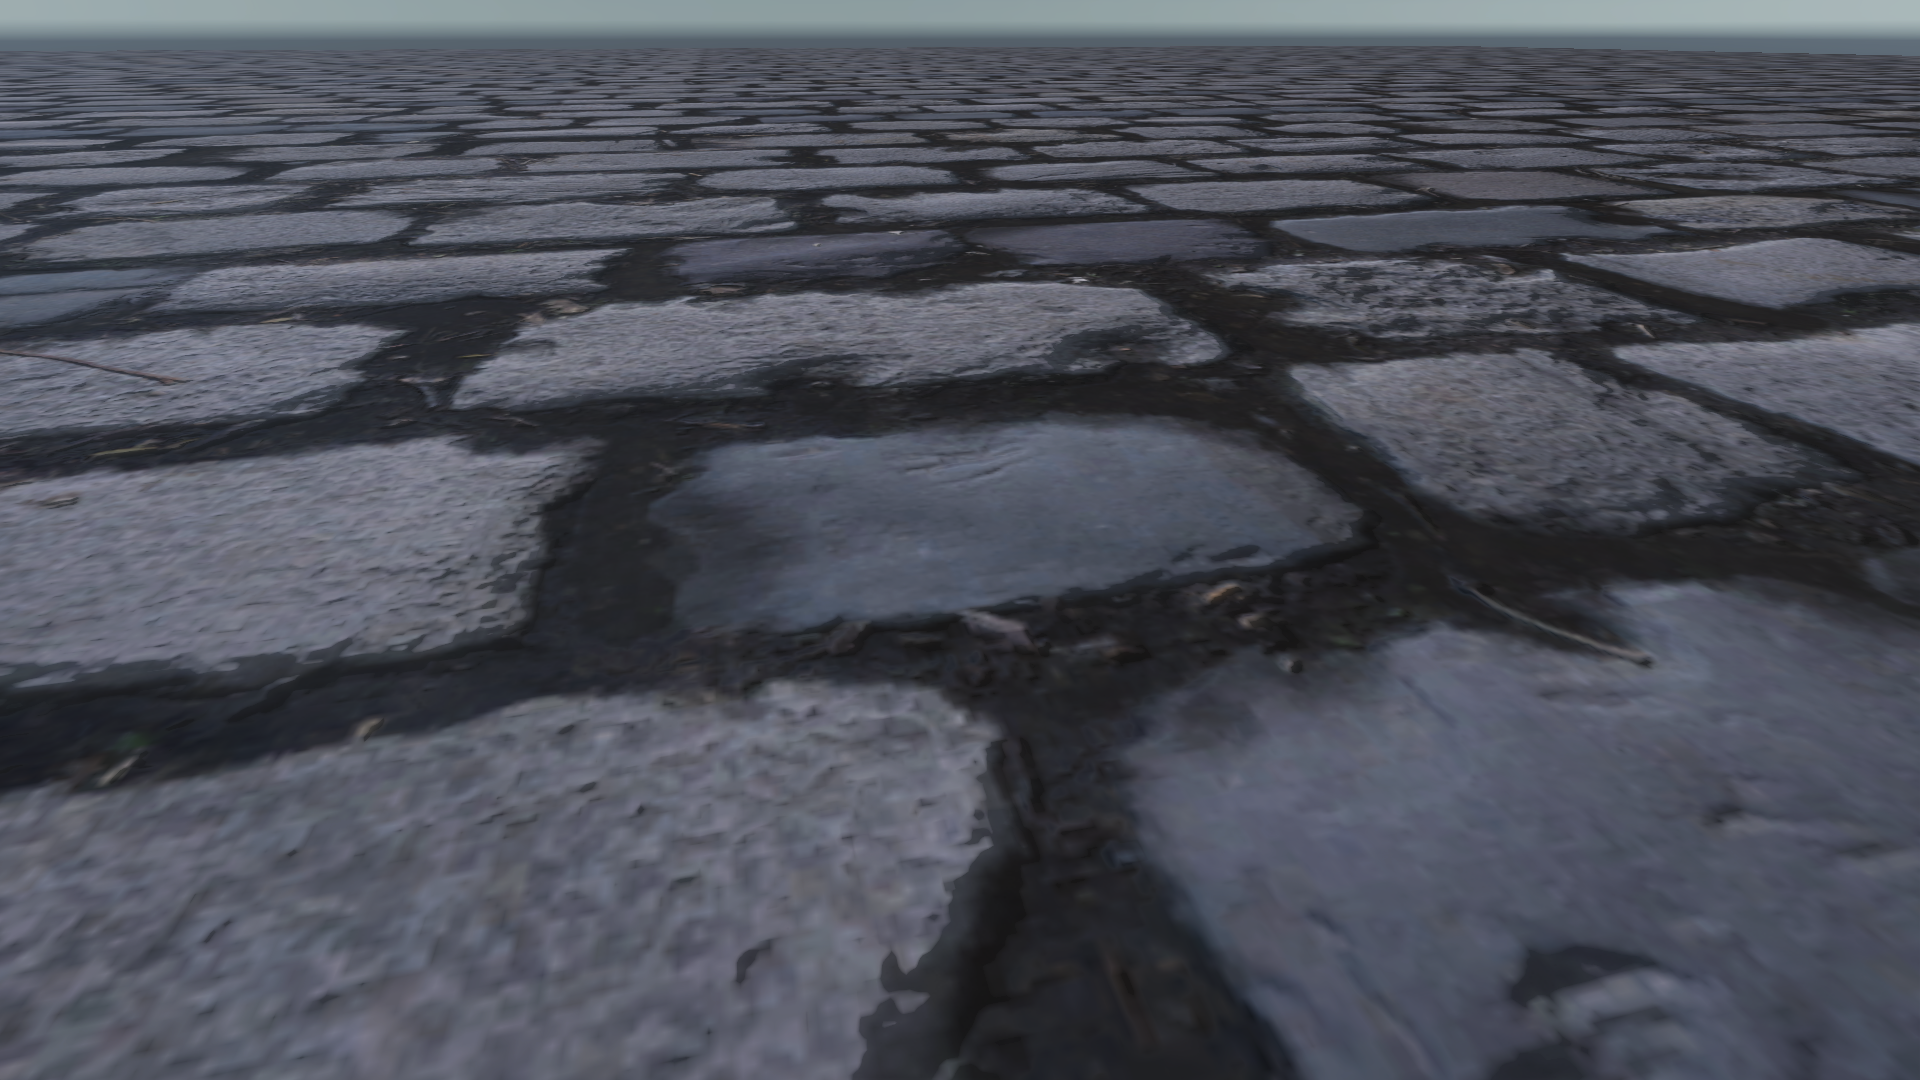
\includegraphics[width=0.49\textwidth]{Grafiken/Basics/Mapping/Vergleich_Normal.png}
	\begin{footnotesize}
		\caption{links: Einfache diffuse Beleuchtung der Textur, rechts: Normal Mapping. Beide Geometrien sind komplett flach. 
		Hierbei sieht man gut den Unterschied zwischen dem flachen Look
		der diffus beleuchteten Textur und dem realistischeren Aussehen durch Einbeziehen der Oberflächennormalen aus der Normal Map.}
	\end{footnotesize}
\end{figure}

\subsubsection{Displacement Mapping}
Mit Displacement Mapping werden dagegen tatsächlich mithilfe von Heightmaps die Positionen
der Vertices entlang ihrer Normalen versetzt \parencite{Cook1984,Cook1987}. Dadurch kommt es nicht zu blickwinkelabhängigen Artefakten
und die Illusion von Tiefe wird real. Objekte sehen aus einem flachen Winkel betrachtet nicht mehr
glatt aus, sondern haben tatsächlich Struktur in ihrer Oberfläche. Damit dieser Effekt jedoch zustande kommt,
muss das Mesh in einer gewissen Auflösung zur Verfügung stehen. Je nach Detailreichtum der Heightmap
muss die Geometrie dabei in weitere Polygone unterteilt werden. Der Vorteil hierbei ist der hohe
Grad an Realismus. Ein deutlicher Nachteil liegt dabei allerdings in der Performance.
Ein weitgehender Einsatz von Displacement Mapping kann eine hohe Polygonanzahl schnell
negativen Einfluss auf die Renderingzeiten nehmen. 

\textcolor{red}{>>PERFORMANCEVERGLEICH MAPPINGVARIANTEN<<}
\href{https://onlinelibrary.wiley.com/doi/abs/10.1111/cgf.13656}{Hier der Vergleich, TH-VPN nötig}

\subsubsection{Parallax Mapping}

Parallax Mapping (oder auch Offset (Bump-)Mapping) ist eine weiter Methode, um sich die Möglichkeiten von
Bump Mapping-Verfahren zu nutze zu machen. Anders als bei tatsächlicher Modifizierung der Vertices
durch Displacement Maps werden hier nur die Texturkoordinaten abhängig vom Blickwinkel verschoben. \parencite{Kaneko2001, Welsh2004}
Durch Bewegung der Oberfläche oder des Betrachters entsteht somit ein realistischerer Eindruck
von Tiefe in der Textur, welcher den des Displacement Mappings approximiert darstellt.
Dabei ist Parallax Mapping allerdings immer noch deutlich effizienter als echtes Vertex-Displacement
und eignet sich daher eher für Echtzeitrenderings.
Parallax Mapping alleine simuliert zwar den Parallax-Effekt, jedoch ist es hiermit nicht Möglich die Silhoutte zu verändern und
Selbstschattierung oder -verdeckung vorzutäuschen.


\subsubsection{Parallax Occlusion Mapping}
\label{sec:3.3.4}

\begin{figure}[h]
	\centering
	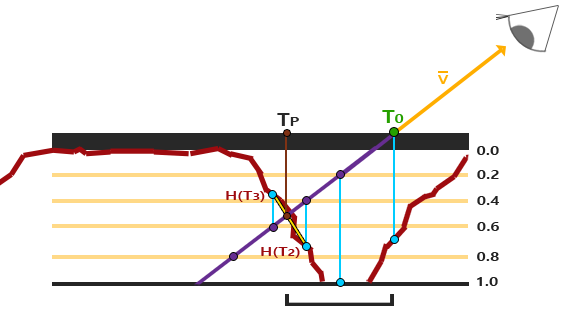
\includegraphics[width=0.8\textwidth]{Grafiken/Basics/Mapping/Infografik_POM.png}
	\begin{footnotesize}
		\caption{Verschiebung der Texturkoordinaten beim Parllax Occlusion Mapping}
	\end{footnotesize}
\end{figure}


Parallax Occlusion Mapping (POM) ist eine komplexere, verbesserte Variante des Parallax Mapping, basierend auf einem Per-Pixel Ray Tracing.
Das Ziel ist auch hier wieder das vorherige: Detaillierte Oberflächen ohne den Preis von teuren Vertexverschiebungen.
Diese Details lassen sich abhängig vom Blickwinkel aus jeder Perspektive korrekt darstellen.
Mithilfe von dynamischer Beleuchtung und Selbstokklusion kann außerdem eine korrekte Selbstschattierung simuliert werden \parencite{Brawley2004, Tatarchuk2006}.
Die Informationen aus der Heightmap werden hierbei für Berechnungen im Fragmentshader verwendet.
Anstatt wie beim Displacement Mapping Details zu extrudieren wird bei POM in die Tiefe simuliert.
Hierbei wird die Oberfläche der Wert 1.0, und damit der höchste Punkt, angenommen.
Zunächst wird für jeden zu rendernden Pixel mittels Ray Castings vom Betrachter zur Geometrie-Oberfläche ein Schnittpunkt  $T_0$ ausfindig gemacht.
Der Strahl $\vec{v}$ wird nun weiter durch das, durch die Heightmap ausgedrückte, Volumen verfolgt und Schrittweise gesampled. Wenn sich der Strahl 
mit der Heightmap im Punkt $T_P$ schneidet
kann mit der Position die neue zu rendernde Texturkoordinate ermittelt werden. Je geringer die Schrittweite ist, desto genauer kann die Oberfläche gerendert werden.
Ist die Schrittgröße zu groß kann die Heightmap nicht detailliert genug abgetastet werden und es entstehen Aliaseffekte, es zeichnet sich
ein Treppeneffekt ab
(\autoref{fig:alias}).


\begin{figure}[ht]
	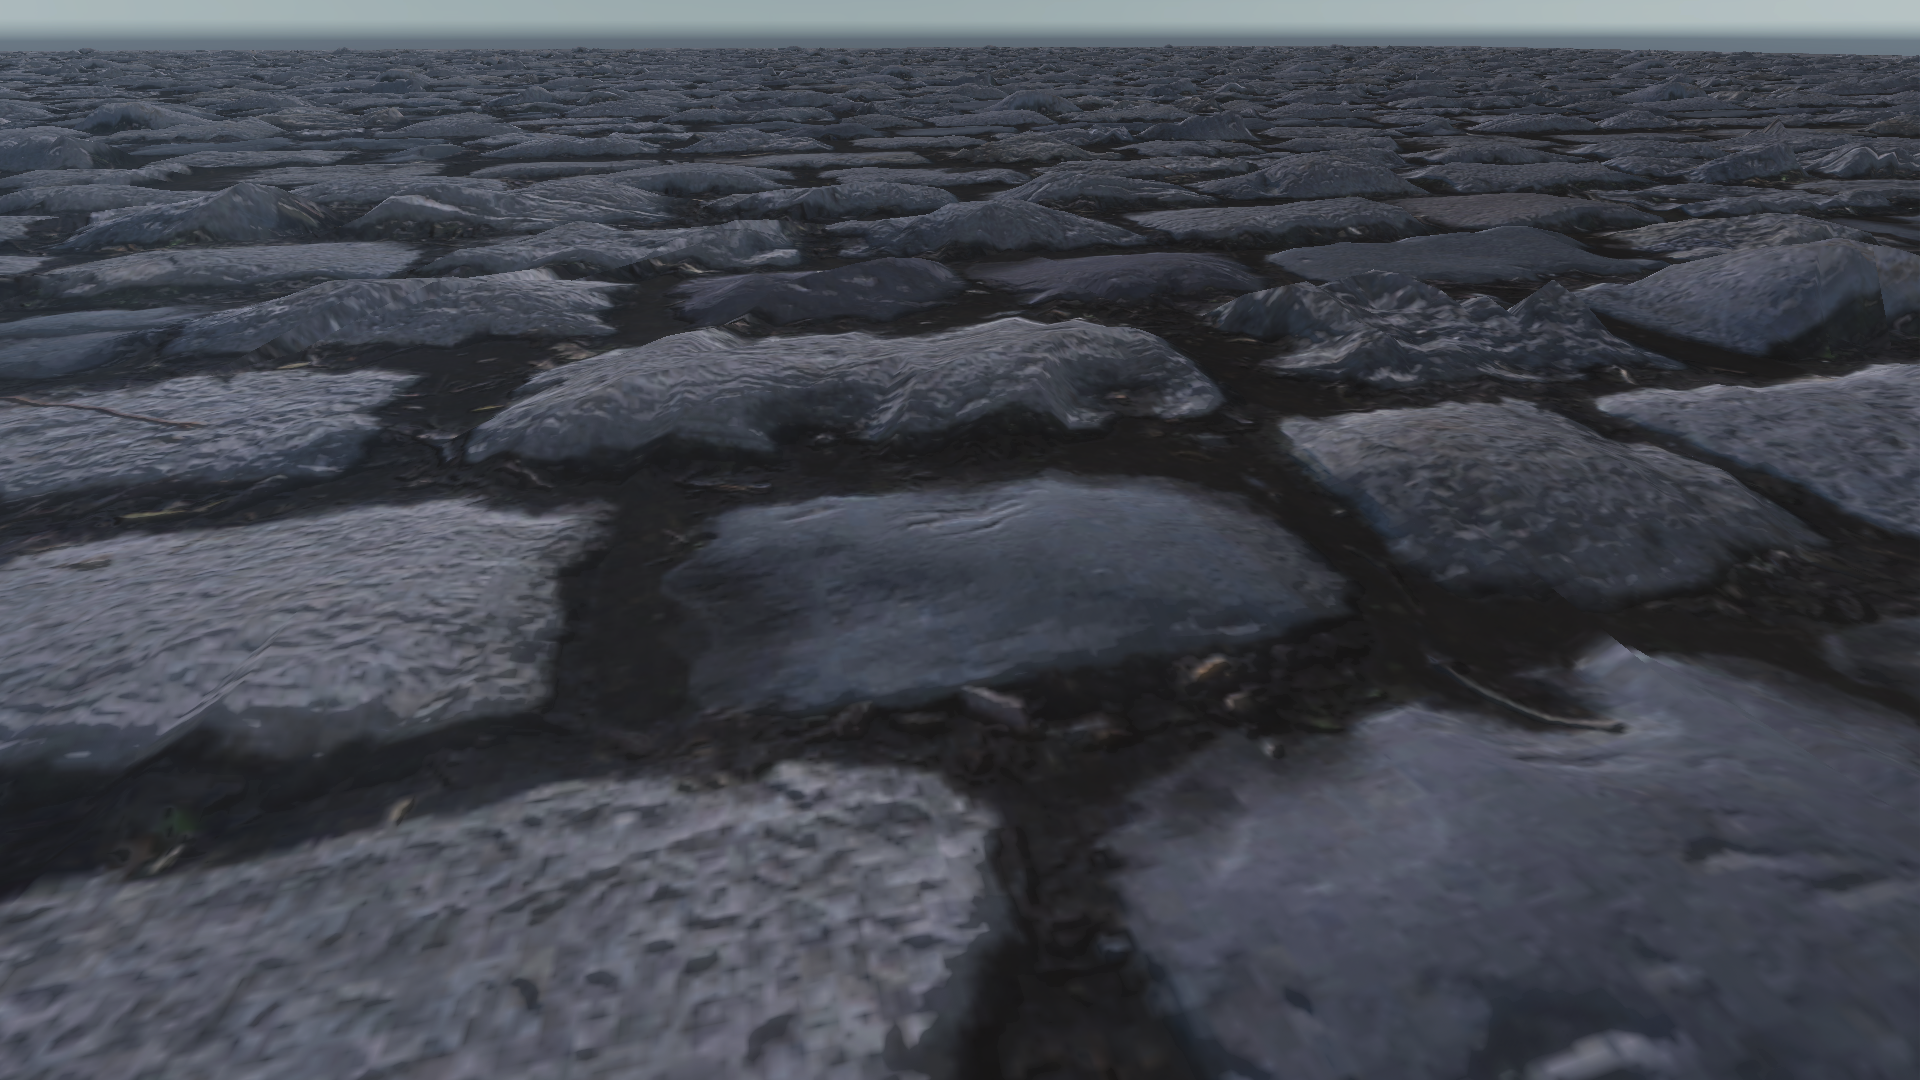
\includegraphics[width=0.49\textwidth]{Grafiken/Basics/Mapping/Vergleich_DisplacementNormalTesselated.png}
	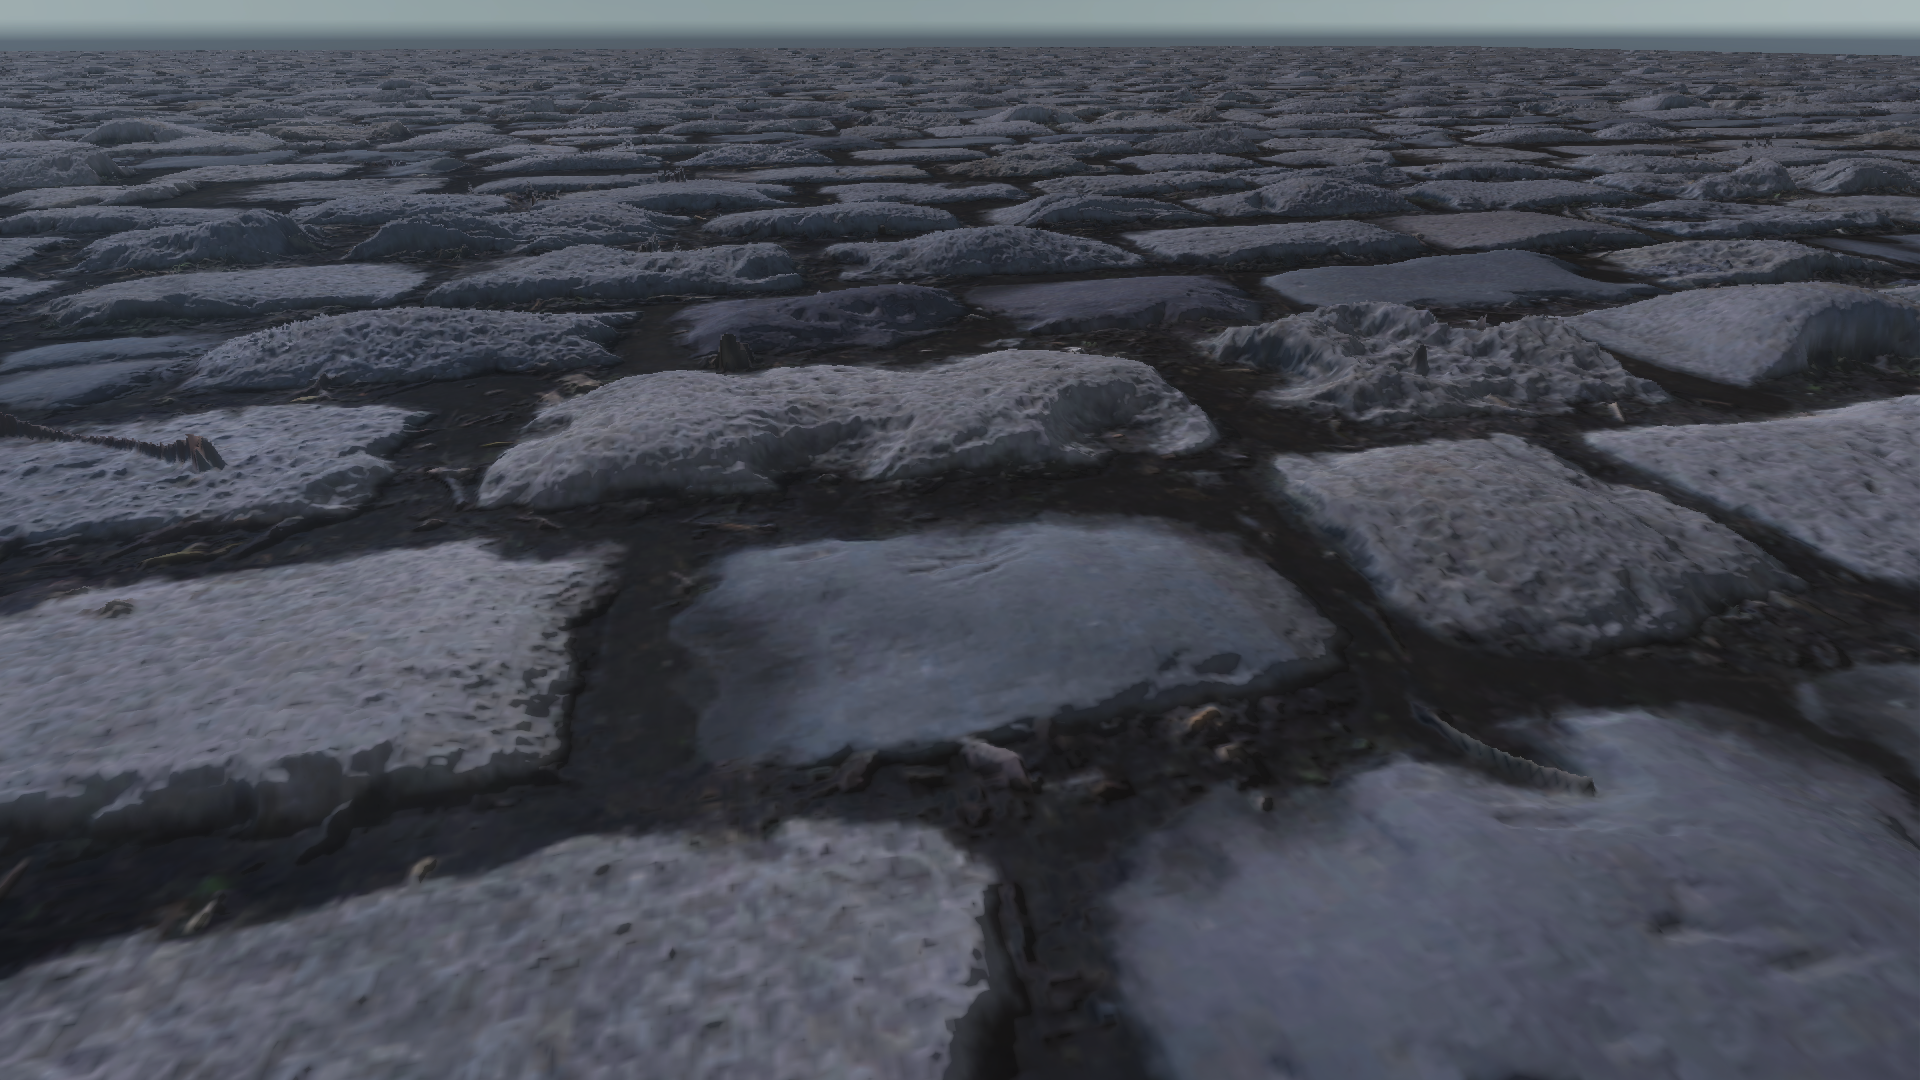
\includegraphics[width=0.49\textwidth]{Grafiken/Basics/Mapping/Vergleich_POM_64Steps.png}
	\begin{footnotesize}
		\caption{links: Displacement Map, Normal Map und 50-facher Tesselation, rechts: Parallax Occlusion Mapping mit 64 Samples. 
		Beide Methoden sehen sich sehr ähnlich, der Unterschied ist jedoch, dass für die Displacement Map-Methode in diesem Beispiel die 50-fache Anzahl an
		Dreiecken gebraucht wird.}
	\end{footnotesize}
\end{figure}


\begin{figure}[h]
	\centering
	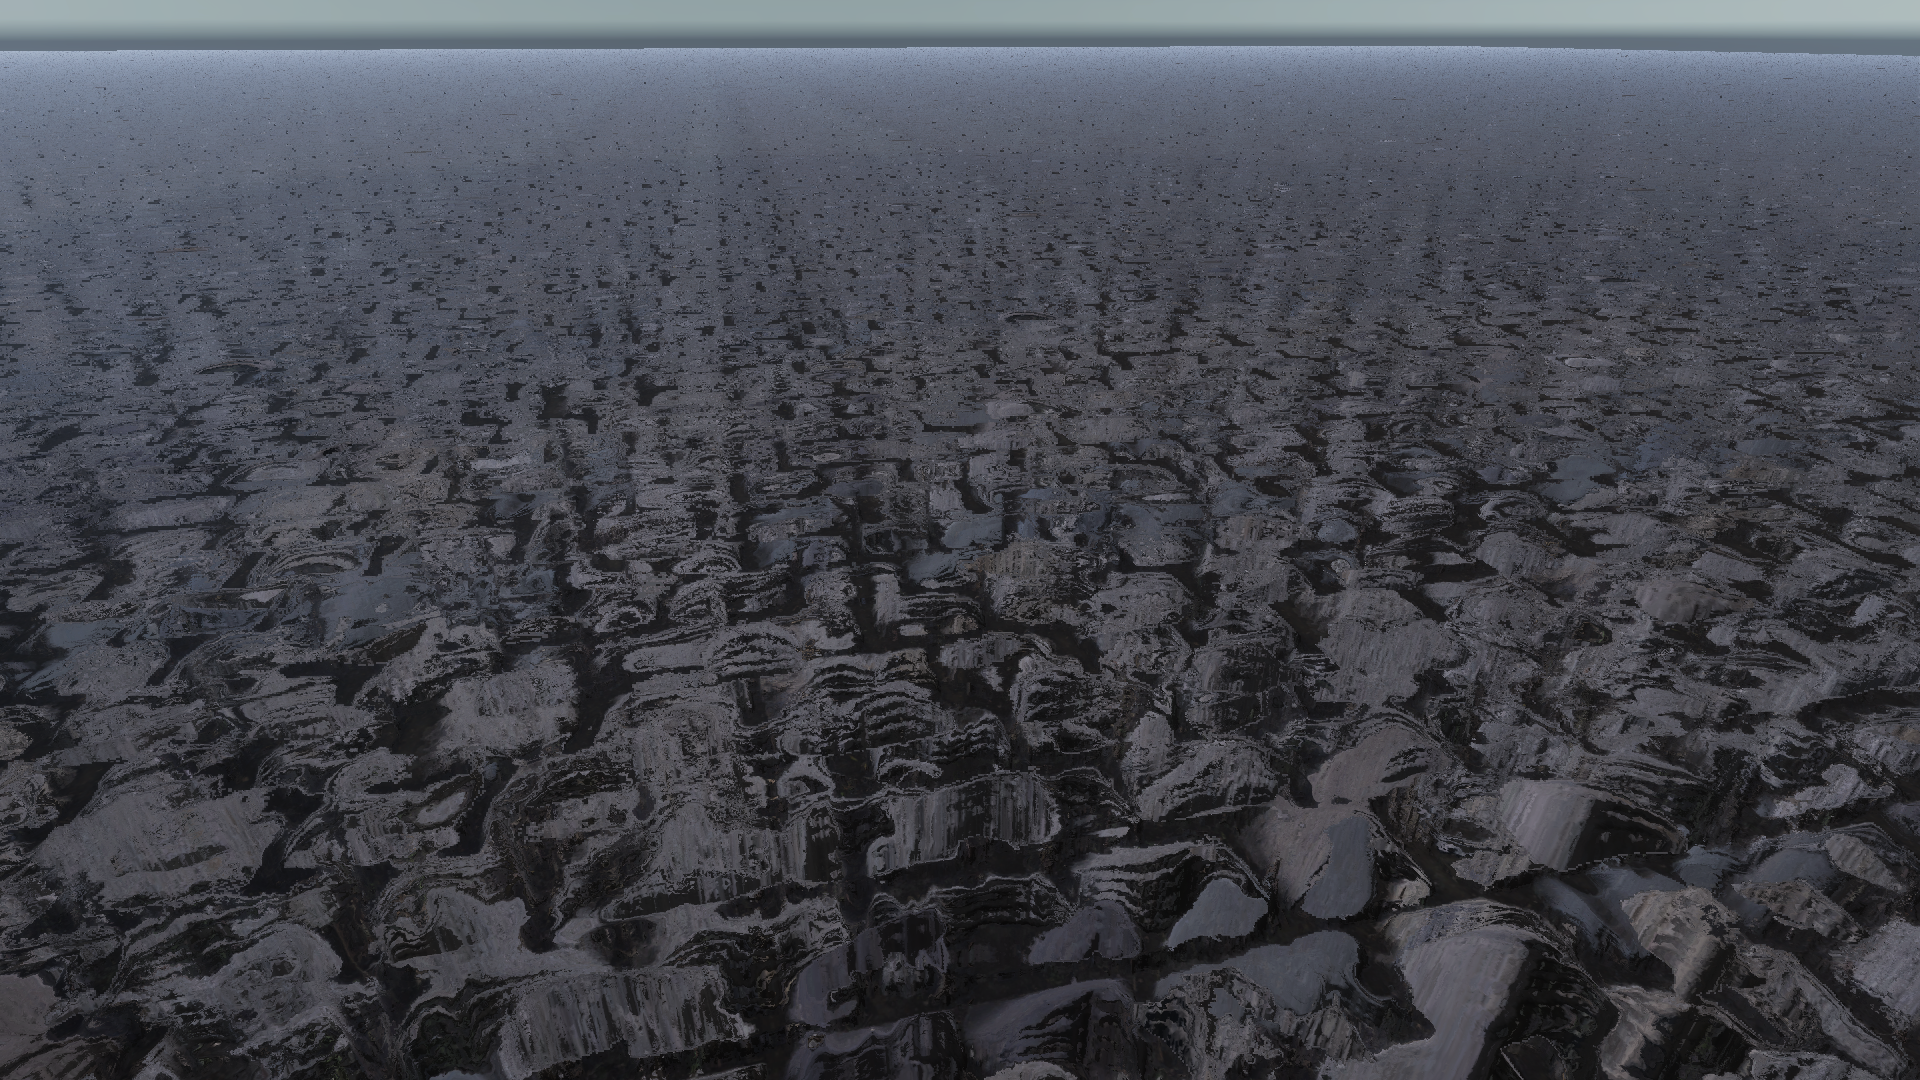
\includegraphics[width=1\textwidth]{Grafiken/Basics/Mapping/aliasing.png}
	\begin{footnotesize}
		\caption{Aliasingeffekt bei zu geringer Sampleanzahl mit 4 Schritten}
		\label{fig:alias}
	\end{footnotesize}
\end{figure}
